\chapter{{\ifpdf{OMDoc}\else{\omdoc}\fi} Applications, Tools,  and Projects}\label{chap:processing}\label{chap:projects}

In this chapter we will address current applications, tools and projects using the
{\omdoc} format.  We will first discuss the possibilities and tools of processing
documents in the {\omdoc} format via stylesheets with the purpose of generating
documents specialized for consumption by other mathematical software systems, and
by humans. Then we will present three projects descriptions that use {\omdoc} at
the core. The {\qmath} project described in section~\ref{sec:qmath} defines an
interface language for a fragment of {\omdoc}, that is simpler to type by hand,
and less verbose than the {\omdoc}, that can be generated by the {\tt{qmath}}
batch processor. The {\mbase} system in section~\ref{sec:mbase} is a a web-based
mathematical knowledge base that offers the infrastructure for a universal,
distributed repository of formalized mathematics represented in the {\omdoc}
format. Finally, the {\activemath} projects described in
section~\ref{sec:activemath} uses the {\omdoc} infrastructure in an educational
setting. It makes use of the content-orientation and the explicit structural
markup of the mathematical knowledge to generate on the fly specialized learning
materials that are adapted to the students prior knowledge, learning goals, and
notational tastes.

The applications of {\omdoc} are not limited to the ones described in this
chapter, in fact there is research and tool development where {\omdoc} is used in
the role of 
\begin{itemize}
\item a {\emin{communication standard}} between mechanized reasoning systems,
  e.g. the {\clam}-{\hol} interaction~\cite{BouSli:aibcah98}, or the
  {\OMEGA}-{\tps}~\cite{BeBiSo:itao99} integration.
\item a data format that supports the {\emin{controlled refinement}} from informal
  presentation to formal specification of mathematical objects and theories.
  Basically, an informal textual presentation can first be marked up, by making
  its structure\index{structure!discourse} explicit (classifying text fragments as
  definitions, theorems, proofs, linking text, and their relations), and then
  formalizing the textually given mathematical knowledge in logical formulae (by
  adding {\element{FMP}} elements; see section~\ref{sec:properties}.
\item an interface language of a {\emin{mathematical knowledge
      base}}\index{knowledge base} like the {\mbase}
  system~\cite{FraKoh:sdmaomkb00,KohFra:rkcimss00}. The system offers a service
  that allows to store and (flexibly) reproduce (parts of) {\omdoc} documents.
\item a {\emin{document preparation language}}; a system like {\mbase} supports the
  maintenance of large-scale document- and conceptual structures, if they are made
  explicit in {\omdoc}. As {\omdoc} can directly be transformed to e.g.
  {\xhtml}+{\mathml}, or {\LaTeX}, external input to {\mbase} can directly be
  published.
\item a basis for {\emph{individualized (interactive)
      books}}\index{book!interactive}\index{individualized book}.  Personalized
  {\omdoc} documents can be generated from {\mbase} making use of the
  {\indextoo{discourse structure}}\index{structure!discourse} encoded in {\mbase}
  together with a user model.
\item an interface for {\emin{proof
      presentation}}~\cite{HuangFiedler:pvip97,Fiedler:uacatp99}: since the proof
  part of {\omdoc} allows small-grained interleaving of formal ({\element{FMP}})
  and textual ({\element{CMP}}) presentations in multiple languages. 
\end{itemize}

Note that the material discussed in this chapter is under continuous development,
and the account here only reflects the state of December 2001, see
{\url{http://www.mathweb.org/omdoc}} for more and current information. The text in
in the project descriptions has been contributed by the authors marked in the
section headings, for questions about the projects or systems, please visit the
web-sites given in the section headings or contact the authors directly.


\ifpdf\section{Transforming OMDoc by XSLT Style Sheets}
\else\section{Transforming {\omdoc} by {\xslt} Style Sheets}\fi
\label{sec:transform-xsl}

In the introduction we have stated that one of the design intentions behind
{\omdoc} is to separate content from presentation, and leave the latter to the
user. In this section, we will briefly touch upon presentation issues. The
technical side of this is simple: {\omdoc} documents are regular {\xml} documents
that can be processed by an {\xslt} {\indextoo{style sheet}} to produce other
formats from {\omdoc} representations. In this section we will review a set of
{\xslt} style sheets that are distributed with {\omdoc}, they can be found in
{\url{http://www.mathweb.org/omdoc/xsl}}.

There are several high-quality {\xslt} transformers freely available
(e.g.  {\ttin{saxon}} ({\url{http:saxon.sourceforge.net}}) or
{\ttin{xalan}} ({\url{http://xml.apache.org/xalan-j}})).  Moreover,
{\xslt} is natively supported by the newest versions of the primary
{\indextoo{browser}}s {\msie}\index{internet@{\msie}} and
{\netscape}\index{netscape@{\netscape}} (see~{\url{http://www.mozilla.org}} for
{\mozilla}\index{mozilla@{\mozilla}}, the open source version).

{\xslt} style sheets can be used for several tasks in maintaining {\omdoc}, such as
for instance converting other {\xml}-based input formats into {\omdoc} (e.g.
{\ttin{cd2omdoc.xsl}} for converting {\openmath} content
dictionaries\index{content dictionary} into {\omdoc} format), or migrating between
different versions of {\omdoc} e.g. the style sheet {\ttin{omdoc1.0adapt1.1.xsl}}
that operationalizes all the syntax changes from {\omdoc} version 1.0 to version
1.1 (see appendix~\ref{sec:changelog} for a tabulation).

\subsection{{\ifpdf{OMDoc}\else{\omdoc}\fi} Interfaces for Mathematical Software
  Systems}\label{sec:omdoc2sys}

One of the original goals of the {\openmath}, {\mathml} and {\omdoc} languages is
to provide a communication language for mathematical software systems. The main
idea behind this is to supply systems with interfaces to a universally accepted
communication language standard (an {\indextoo{interlingua}}), and so achieve
interoperability for $n$ systems with only $2n$ translations instead of $n^2$. As
we have seen in section~\ref{sec:math-objects}, {\openmath} and content {\mathml}
provide a good solution at the level of mathematical objects, which is sufficient
for systems like computer algebra systems. {\omdoc} adds the level of mathematical
statements and theories to add support for automated reasoning systems and formal
specification systems.

To make practical use of the {\omdoc} format as an interlingua, we have to support
building {\omdoc} interfaces. An {\xslt} style sheet is a simple way to come up
with (the input half) of an {\omdoc} interface, a more efficient way would be to
integrate an {\xml}\index{xml@{\xml} parser} parser\index{parser!{\xml}} directly
into the system (suitable {\xml} parsers are readily available for almost all
programming languages now).

Usually, the task of writing an {\xslt} style sheet for such a conversion is a
relatively simple task, since the input language of most mathematical software
system is isomorphic to a subset of {\omdoc}. This suggests the general strategy
of applying the necessary syntax transformations (this has to be supplied by the
style sheet author) on those {\omdoc} elements that carry system-relevant
information and transforming those that are not (e.g. Metadata and {\element{CMP}}
elements for most systems) into comments.  Much of the functionality is already
supplied by the style sheet {\ttin{omdoc2sys.xsl}}, which need only be adapted to
know about the comment syntax. For examples see the {\ttin{omdoc2pvs.xsl}} style
sheet that transforms {\omdoc} to {\pvs} input.

The other direction of the translation needed for communication is
usually much more complicated, since it involves parsing the often
idiosyncratic output of these systems. A better approach (which we
followed with the systems above) is to write specialized output
generators for these systems that directly generate {\omdoc}
representations. This is usually a rather simple thing to do, if the
systems have internal data structures that provide all the information
required in {\omdoc}. It is sometimes a problem with these systems
that they only store the name of a symbol (logical constant) and not
its home theory. At other times it internal records of proofs in
theorem provers are optimized towards speed and not towards
expressivity, so that some of the information that had been discarded
has to be recomputed for {\omdoc} output.

One of the practical problems that remains to be solved for interfaces to
mathematical software systems is that of semantical standardization of input
languages. For mathematical objects, this has been in principle solved by
supplying a theory level in the form of {\openmath} content dictionaries or
{\omdoc} documents that define the necessary mathematical concepts. For systems
like theorem provers or theory development environments this has not been done
yet. 

{\omdoc} can help with this task, as we have seen in series of
experiments of connecting the theorem proving systems
{\OMEGA}~\cite{BenzmuellerEtAl:otama97}, {\inka}~\cite{HuSe:itng96},
{\pvs}~\cite{OwRu92}, {\lambdaclam}~\cite{RicSmaGre:ppihol98},
{\tps}~\cite{AnBi:tatps96} and {\coq}~\cite{CoqManual} to the {\mbase}
system by equipping them with an {\omdoc} interface.

The first observation in the interpretation is that even though the systems are of
relatively different origin, their representation languages share many features
\begin{itemize}
\item {\tps} and {\pvs} are based on a simply typed $\lambda$-calculus, and only
  use type polymorphism in the parsing stage, whereas {\OMEGA} and {\lambdaclam}
  allow ML-style type polymorphism.
\item {\OMEGA}, {\inka} and {\pvs} share a higher sort concept, where sorts are
  basically unary predicates that structure the typed universe.
\item {\pvs} and {\coq} allow dependent- and record types as basic
  representational features. 
\end{itemize}
but also differ on many others
\begin{itemize}
\item {\inka}, {\pvs}, and {\coq} explicitly support inductive definitions, but by
  very different mechanisms and on differing levels.
\item {\coq} uses a constructive base logic, whereas the other systems are classical.
\end{itemize}
At one level, the similarities are not that surprising, all of these systems come
from similar theoretical assumptions (most notably the Automath
project~\cite{Bruijn80}), and inherit the basic setup (typed $\lambda$ calculus)
from it. The differences can be explained by differing intuitions in the system
design and in the intended applications.

Following recent work on the systemization and classification of $\lambda$-calculi
{\cite{Barendregt:lcwt92}}, we have started to ground these languages in language
hierarchy. The structural similarities between theories and logical languages and
their structuring morphisms allow to re-use the {\omdoc}/{\mbase} theory mechanism
for language definition: The logical symbols and language constructs can be
defined just like other (object-level) symbols/concepts. As a consequence, the
development of the {\omdoc} interface to the theorem provers mentioned above
included the specification of the representation language as a theory (which could
be used as an integrated documentation). The structured theory mechanism can now
be used to re-use and inter-relate the various representation formats between the
theorem provers. For instance the simply typed $\lambda$-calculus can be factored
out (and thus shared) of the representation languages of all of the theorem
proving systems above. This makes the exchange of logical formulae via the
{\omdoc} format very simple, if they happen to be in a suitable common fragment:
In this case, the common ({\openmath}/{\omdoc}) syntax is sufficient for
communication.

\subsection{Presenting {\ifpdf{OMDoc}\else{\omdoc}\fi} to Humans}\label{sec:omdoc2pres}

One of the main goals of content markup for mathematical documents is to be
independent of the output format. In the last chapter, we have specified the
conceptual infrastructure provided by the {\omdoc} language, in this section we
will discuss the software infrastructure needed to transform {\omdoc} documents
into human-readable form in various formats. We speak of of {\omdoc}
{\defin{presentation}} for this task.

Due to the complex nature of {\omdoc} presentation, only part of it
can actually be performed by {\xslt} style sheets. For instance,
subtasks like reasoning about the prior knowledge of the user, or her
experience with certain proof techniques is clearly better left to
specialized applications. Our processing model is the following:
presenting an {\omdoc} is a two-phase process. The first one is
independent of the final output format (e.g. {\html}, {\mathml}, or
{\LaTeX}) and produces another {\omdoc} representation specialized to
the respective user or audience, taking into account prior knowledge,
structural preferences, bandwidth and time constraints, etc.  This is
followed by a formatting process that can be done by {\xslt} style
sheets that transforms the resulting specialized document into the
respective output format with notational- and layout preferences of
the audience. We will only discuss the second one and refer the reader
for ideas about the first process to systems like
P.rex~\cite{Fiedler:ddaoeo01,FiedlerHoracek:aietlp01}.

At the moment, we have {\xslt} style sheets to convert {\omdoc} to {\html},
presentation {\mathml}, and {\LaTeX}, they can be found at
{\url{http://www.mathweb.org/omdoc/xsl}}.  They consist of two parts: a generic
part that implements the presentation decision for the {\omdoc} (and {\openmath})
elements, and a theory-specific part for the presentation of {\openmath} symbols.

The first part is carried out by the style sheets {\ttin{omdoc2html.xsl}} for
{\html} and and {\ttin{omdoc2tex.xsl}} for {\LaTeX}. They share a large common
code base {\ttin{omdoc2share.xsl}}, basically the first two include the latter and
only redefine some format-specific options. For instance, {\ttin{omdoc2share.xsl}}
supplies an infrastructure for {\indextoo{internationalization}}. In
section~\ref{sec:properties} we have introduced multilingual
groups\index{multilingual
  support}\index{support!multilingual}\index{languages!multiple} of
{\element{CMP}} elements. This allows to generate localized presentations of the
{\omdoc} documents, if enough information is present. {\ttin{omdoc2share.xsl}}
takes a {\indextoo{parameter}} {\ttin{TargetLanguage}}, whose value can be a
whitespace-separated preference list of {\indextoo{ISO 639}} two-letter
{\indextoo{country code}s}\index{code!country}. If {\ttin{TargetLanguage}} consists
of a single entry, then the result will only contain this language with gaps where
the source document contains no suitable {\element{CMP}}. Longer
{\ttin{TargetLanguage}} preference lists will generally result in more complete
documents. Apart from the language-specific elements in the source document,
{\indextoo{localization}} also needs to know about the presentation of certain
keywords used in {\omdoc} markup, e.g.  the German ``Lemma'' and the French
``Lemme'' for \verb+<assertion type="lemma">+. This information is kept in the
keyword table {\url{http://www.mathweb.org/omdoc/lib/locale.xml}}, which contains
all the keywords necessary for presenting the {\omdoc} elements discussed so far.
An alternative keyword table can be specified by the parameter
{\index{parameter!{\xslt}}} {\tt{locale}}\index{locale@{\tt{locale}} ({\xslt}
  parameter)}.

Presentation of {\openmath} symbols in formulae is a process based on the
presentation information described in section~\ref{sec:presentation} to re-create
their typographic conventions in the output format. To present a file
{\tt{test.omdoc}} in e.g. {\html}, we first generate an {\xslt} style sheet
{\tt{test2html.xsl}} and the apply it to {\tt{test.omdoc}} to generate the {\html}
file {\tt{test.html}}. Note that {\tt{test2html.xsl}} needs to include specific
{\xslt} templates for all symbols that are used in formulae, so
{\tt{test2html.xsl}} includes the three style sheets 
\begin{description}
\item[{\ttin{omdoc2html.xsl}}] for presentation of the {\omdoc} elements that are
  not symbols.
\item[{\tt{test4html.xsl}}] a style sheet that contains templates for symbols that
  are are defined in {\tt{test.omdoc}}, it is generated by applying an {\xslt}
  meta-stylesheet {\ttin{expres.xsl}} with parameter {\ttin{format}} =
  {\ttin{html}} to {\tt{test.omdoc}}. Concretely, if {\tt{test.omdoc}} defines the
  symbol {\tt{forall}} and contains the {\element{presentation}} element in
  {\myfigref{ombind-presentation}} (page~\pageref{fig:ombind-presentation}), then it
  generates an {\xslt} style sheet {\url{fol4html.xsl}} that contains the template
  in {\myfigref{template}} (page~\pageref{fig:template}).
\item[{\tt{omdocIhtml.xsl}}] this is a style sheet that provides templates for all
  symbols that are used but not defined in {\tt{test.omdoc}}. Concretely this is
  just a list of {\xslt} {\tt{xsl:include}} statements that include style sheets
  {\tt{xxx4html.xsl}} extracted by {\ttin{expres.xsl}} from files {\tt{xxx.omdoc}}
  that define symbols used in formulae in {\tt{test.omdoc}}. We use the style
  sheet {\ttin{exincl.xsl}} parameter {\ttin{format}} = {\ttin{html}} to generate
  {\tt{testIhtml.xsl}} from {\tt{test.omdoc}}.
\end{description}
This two-level approach to notation presentation in {\omdoc} provides a maximum of
flexibility and locality in information management.

\begin{projectdescription}
  \ifpdf\section{QMath: An Authoring Tool for OMDoc}
\else\section{{\qmath}: An Authoring Tool for {\omdoc}}\fi\label{sec:qmath}
\begin{center}\large\sf Alberto Gonz\'alez Palomo\\
\url{http://www.matracas.org}
\end{center}

{\qmath} is a batch processor that produces an {\omdoc} file from a plain Unicode
text document. The purpose of {\qmath} is to allow fast writing of mathematical
documents, using plain text and a straightforward syntax (like in computer algebra
systems) for mathematical expressions .

The ``Q'' was intended to mean ``quick'', since {\qmath} began in 1998 as an
abbreviated notation for {\mathml}. The first version (0.1) just expanded the
abbreviations to full {\mathml} element names, and added the extra markup such as
{\tt{<mrow>}} and the like.  There have been many changes (and two complete
rewrites) since then. You can find a more detailed history at
{\url{http://www.matracas.org/qmath/history.html}}

{\qmath} is very simple in its design: it just parses a text (UTF-8) file
according to a user-definable table of symbols, and builds an XML document from
that. The symbol definitions are grouped in files called ``contexts''. The idea is
that when you declare a context, its file is loaded and from then on these symbol
definitions take precedence over any previous one, thus setting the context for
parsing of subsequent expressions.

The text is split into ``paragraphs'', which are pieces of text separated by at
least one empty line. Each paragraph can have a metadata section at the beginning.
There are a variety of classes of paragraphs, which are identified by a name
followed by a colon (``:''), optionally followed by an identifier which becomes
the {\attribute{id}{*}} attribute of the generated {\omdoc} element. The text is
put in a {\tt{<CMP>}} inside a container element which depends on the paragraph
type. This can be anything allowed by {\omdoc}, such as {\tt{<assertion>}} ,
{\tt{<axiom>}}, or the default {\tt{<omtext>}} if the paragraph doesn't have a
{\qmath} paragraph type label. Inside the text, a mathematical expression is
enclosed in dollar (``{\tt{\$}}'') signs.  Each such a section becomes an
{\element{OMOBJ}} element in the output document.

\begin{myfig}{qmathex}{A minimal {\qmath} document and its {\omdoc} result}\scriptsize
\begin{boxedverbatim}
QMATH 0.3.6
:"Diary"
:Winston Smith
:1984-04-04
:en

Context: "Mathematics/Arithmetic"
Context: "Mathematics/OMDoc"

Theory:[<-thoughtcrime]

:"Down with Big Brother"
Freedom is the freedom to say $2+2=4$. 
If that is granted, all else follows.
\end{boxedverbatim}
\quad
\begin{tabular}[b]{|p{5.2cm}|}\hline
From {\url{contexts/en/Mathematics/OpenMath/arith1.qmath}}:\\
{\tt{Symbol: plus OP\_PLUS "arith1:plus"}}\\
{\tt{Symbol: + OP\_PLUS "arith1:plus"}}\\
{\tt{Symbol: sum APPLICATION "arith1:sum"}}\\
{\tt{Symbol: \( \Sigma \) APPLICATION "arith1:sum"}}\\
 $\cdots$\\\hline

From {\url{contexts/en/Mathematics/OpenMath/relation1.qmath}}:\\
{\tt{Symbol: = OP\_EQ "relation1:eq"}}\\
{\tt{Symbol: neq OP\_EQ "relation1:neq"}}\\
{\tt{Symbol: \ensuremath{�}= OP\_EQ "relation1:neq"}}\\
{\tt{Symbol: \( \neq \) OP\_EQ "relation1:neq"}}\\
 $\cdots$\\\hline
\end{tabular}
\\\footnotesize
\begin{boxedverbatim}
<?xml version='1.0' encoding='UTF-8' standalone='no'?>
<!DOCTYPE omdoc PUBLIC "-//OMDoc//DTD OMDoc V1.1//EN" 
                       "http://www.mathweb.org/omdoc/omdoc.dtd" []>
<omdoc lang='en'>
 <metadata lang='en'>
  <Title xmlns='http://purl.org/DC'>Diary</Title>
  <Contributor xmlns='http://purl.org/DC' role='aut'>
   Winston Smith
  </Contributor>
  <Date xmlns='http://purl.org/DC'>1984-04-04</Date>
 </metadata>
 <theory id='thoughtcrime'>
  <omtext>
   <metadata>
    <Title xmlns='http://purl.org/DC'>Down with Big Brother</Title>
   </metadata>
   <CMP>
    Freedom is the freedom to say 
    <OMOBJ xmlns='http://www.openmath.org/OpenMath'>
     <OMA>
      <OMS cd='relation1' name='eq'/>
      <OMA><OMS cd='arith1' name='plus'/><OMI>2</OMI><OMI>2</OMI></OMA> 
      <OMI>4</OMI>
     </OMA>
    </OMOBJ>.
    If that is granted, all else follows. 
   </CMP>
  </omtext>
 </theory>
</omdoc>
\end{boxedverbatim}
\end{myfig}

{\Myfigref{qmathex}} shows a minimal {\qmath} document, and the {\omdoc} document
generated from it.  The first line ("{\tt{QMATH 0.3.6}}") in the {\qmath} document
is required for the parser to recognize the file. The lines beginning with
``{\tt{:}}'' are metadata items: first the document title, then the author name
(one line for each author), and finally the primary language for the document.
This last item is required, as it sets the basic symbol set accordingly. For
example, the ``{\tt{Context}}'' item of an English document is written
``{\tt{Contexto}}'' if the document is in Spanish.  (Similarly, the arithmetic
context would be "{\tt{Matem\'aticas/Aritm\'etica}}") The document is split into
paragraphs, which are separated by empty lines.  Then, mathematical expressions
are written enclosed by ``{\tt{\$}}'' (dollar) signs.

The {\tt{QMath}} command works as a pure filter: reads the document from standard
input, and writes the resulting {\omdoc} in standard output. So, the typical usage
is
\begin{verbatim}
QMath <document.qmath > document.omdoc
\end{verbatim}
It needs the {\tt{QMATH\_HOME}} environment variable to contain the path for the
root {\qmath} directory, where it can find the "contexts" directory. For example,
if you have the {\tt{contexts}} directory at {\url{/tmp/qmath_3/contexts}}, you
should set {\tt{QMATH\_HOME}} to {\url{/tmp/qmath_3}}

{\qmath} is distributed under the GNU General Public License (GPL):
{\url{http://www.gnu.org/licenses/licenses.html#GPL}}

%%% Local Variables: 
%%% mode: latex
%%% TeX-master: "omdoc"
%%% End: 


\end{projectdescription}

\begin{projectdescription}
  \ifpdf\section{MBase, an Open Mathematical Knowledge Base}
\else\section{{\mbase}, an Open Mathematical Knowledge Base}\fi\label{sec:mbase}
\begin{center}\large\sf Andreas Franke and Michael Kohlhase\\
\url{http://www.mathweb.org/mbase}
\end{center}

We describe the {\mbase} system, a web-based mathematical knowledge base
(see~\url{http://www.mathweb.org/mbase}). It offers the infrastructure for a
universal, distributed repository of formalized mathematics. Since it is
independent of a particular deduction system and particular logic, the {\mbase}
system can be seen as an attempt to revive the {\sc Qed} initiative from an
infrastructure viewpoint. See~\cite{KohFra:rkcimss00} for the logical issues
related to supporting multiple logical languages while keeping a consistent
overall semantics. The system is realized as a mathematical service in the
{\mathweb} system~\cite{FraKoh:mabdl99}, an agent-based implementation of a
mathematical software bus for distributed mathematical computation and knowledge
sharing. The content language of {\mbase} is {\omdoc}.

We will start with a description of the system from the implementation point of
view (we have described the data model and logical issues
in~\cite{KohFra:rkcimss00}).  

The {\mbase} system is realized as a distributed set of {\mbase} servers (see
figure~\ref{fig:mbase}). Each {\mbase} server consists of a Relational Data Base
Management System (RDBMS) connected to a {\mozart} process
(yielding a {\mathweb} service) via a standard data base interface.
For browsing the {\mbase} content, any {\mbase} server provides an {\tt
  http} server (see {\url{http://mbase.mathweb.org:8000}} for an example) that
dynamically generates presentations based on {\html} or {\xml} forms.

This architecture combines the storage facilities of the RDBMS with the
flexibility of the concurrent, logic-based programming language
{\oz}~\cite{Smolka:Oz:95}, of which {\mozart} (see
{\url{http://www.mozart-oz.org}}) is a distributed implementation .  Most
importantly for {\mbase}, {\mozart} offers a mechanism called {\defin{pickling}},
which allows for a limited form of persistence: {\mozart} objects can be
efficiently transformed into a so-called pickled form, which is a binary
representation of the (possibly cyclic) data structure.  This can be stored in a
byte-string and efficiently read by the {\mozart} application effectively
restoring the object.  This feature makes it possible to represent complex objects
(e.g. logical formulae) as {\oz} data structures, manipulate them in the {\mozart}
engine, but at the same time store them as strings in the RDBMS. Moreover, the
availability of ``{\oz}lets'' ({\mozart} functors) gives {\mbase} great
flexibility, since the functionality of {\mbase} can be enhanced at run-time by
loading remote functors. For instance complex data base queries can be compiled by
a specialized {\mbase} client, sent (via the Internet) to the {\mbase} server and
applied to the local data e.g. for specialized searching
(see~\cite{Duchier:tntb98} for a related system and the origin of this idea).

\begin{figure}
  \begin{center}
    \ifpdf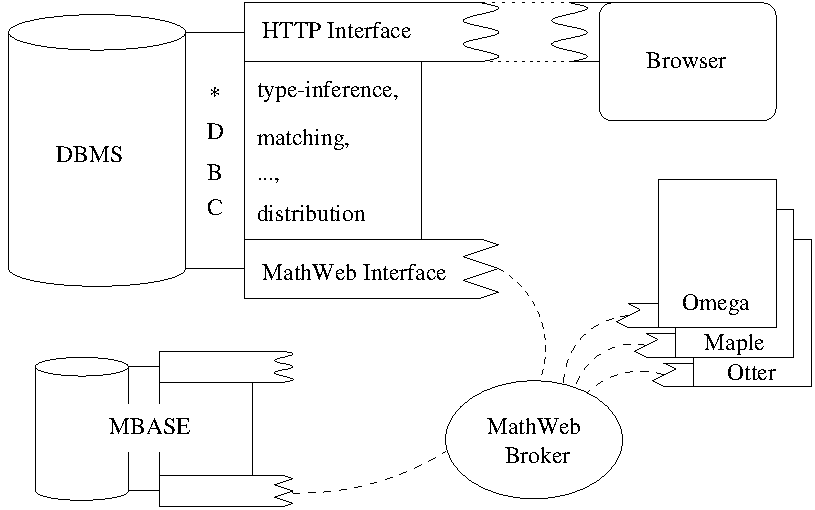
\includegraphics[width=10cm]{mbase.pdf}
    \else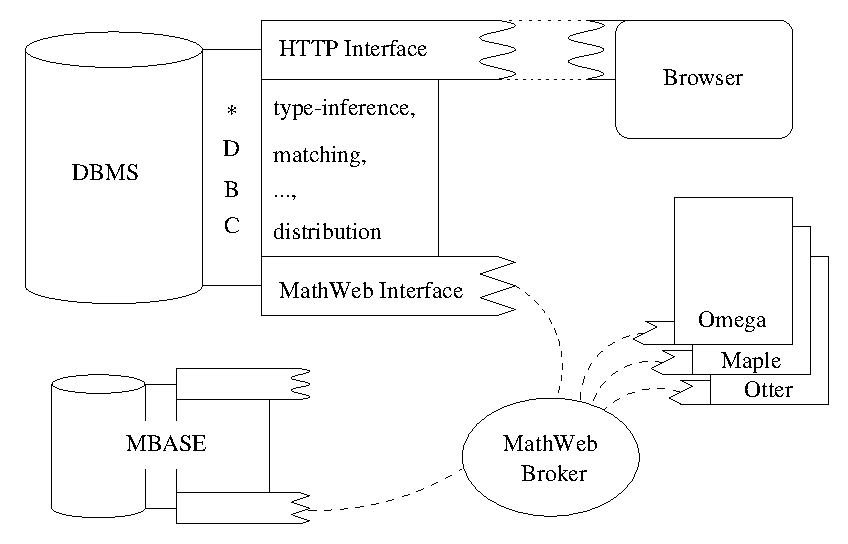
\includegraphics[width=10cm]{mbase.eps}\fi
    \caption{System Architecture}
    \label{fig:mbase}
  \end{center}
\end{figure}

{\mbase} supports transparent distribution of data among several {\mbase} servers
(see~\cite{KohFra:rkcimss00} for details). In particular, an object $O$ residing
on an {\mbase} server $S$ can refer to (or depend on) an object $O'$ residing on a
server $S'$; a query to $O$ that needs information about $O'$ will be delegated to
a suitable query to the server $S'$.  We distinguish two kinds of {\mbase} servers
depending on the data they contain: {\em archive servers\/} contain data that is
referred to by other {\mbase}s, and {\em scratch-pad\/} {\mbase}s that are not
referred to. To facilitate caching protocols, {\mbase} forces archive servers to
be {\em conservative}, i.e. only such changes to the data are allowed, that the
induced change on the corresponding logical theory is a conservative extension.
This requirement is not a grave restriction: in this model errors are corrected by
creating new theories (with similar presentations) shadowing the erroneous ones.
Note that this restriction does not apply to the non-logical data, such as
presentation or description information, or to scratchpad {\mbase}s making them
ideal repositories for private development of mathematical theories, which can be
submitted and moved to archive {\mbase}s once they have stabilized.

%%% Local Variables: 
%%% mode: latex
%%% TeX-master: "omdoc"
%%% End: 

\end{projectdescription}


\begin{projectdescription}
  \section{Project {\ifpdf{ActiveMath}\else{\activemath}\fi}}\label{sec:activemath}
\begin{center}\large\sf
Erica Melis, Eric Andr\`es, Jochen B\"udenbender, Adrian Frischauf,\\
     George Goguadze, Paul Libbrecht, Martin Pollet, Carsten Ullrich\\
\url{http://www.activemath.org/}
\end{center}

In a nutshell, {\activemath} is a generic web-based learning system that
dynamically generates interactive (mathematics) courses adapted to the student's
goals, preferences, capabilities, and knowledge.  The content is represented in
{\omdoc} format with several extensions needed in an educational context. For each
user, the appropriate content is retrieved from the knowledge base {\mbase} and
the course is generated individually according to pedagogical rules.  Then the
course is presented to the user via a standard web-browser. One of the exceptional
features of {\activemath} is its integration of stand-alone mathematical service
systems.

Currently, a minimal authoring kit and a translation tool from restricted {\LaTeX}
to {\omdoc} are provided to support authoring {\omdoc}s\footnote{See
  \url{http://www.activemath.org/~paul/AuthoringComments/} for a description.}.

In the near future, the authoring tools will have intelligent features and
{\activemath} will integrate a user-adaptive suggestion and feedback mechanism in
addition to the adaptive course generation. A comprehensive description of the
system can be found in~\cite{activemathAIEDJ01}.

\subsection{OMDoc Extensions}
The {\activemath} DTD is an extension of the general {\omdoc} DTD, in particular,
with pedagogically motivated extensions such as difficulty or abstractness of an
example or exercise.

{\activemath} will also differentiate exercises according to their type with
values defining the user's required activity such as {\it check-question}, {\it
  make-hypothesis}, {\it prove}, {\it model} or {\it explore} where e.g.,
\textit{explore} means interactive exploration with the help of specified external
system (such as \texttt{maple}, {\OMEGA}, or statistics software).

Additional pedagogically motivated metadata elements will be introduced such as
{\tt field} (e.g., {\it computer science},{\it math}, {\it economy}) and
{\tt{learning\-context}} with values corresponding to school and university
levels\footnote{These will be used to provide different content to users with
  different background fields and at different levels.} in accordance with the
Learning Object Metadata Standard\footnote{\url{http://ltsc.ieee.org/wg12/}}.
Furthermore, the author can specify the pedagogical goal of an exercise, example,
or elaboration, that is whether learning this item increases {\it knowledge}, {\it
  comprehension}, {\it application}, or {\it transfer}.

Finally, in {\activemath}, relations are going to be represented by the element
{\tt relation}, defined in the {\activemath} DTD and classified by introducing a
type of the relation. The type values are: {\it depends-on}, {\it
  counterexam\-ple-for}, {\it similar-example}, {\it similar-exercise}, {\it
  citation}, etc. The need for distinguishing the types of relations arises not
only in educational contexts.

Since we need certain additional {\omdoc} elements in the educational context, a
common representation for proof methods, proof plans, algorithms will be added in
the future, hopefully some of them even to the common {\omdoc} itself.

%??verbosity ?? highlight


\subsection{Adaptive Presentation}

{\activemath} offers dynamically constructed courses that suit the learner's
learning goals, her choosen learning scenarios, her presentation preferences, and
knowledge mastery. To realize this, {\activemath} maintains a user model and its
presentation tools include a course generator and pedagogical rules employed by
the course generator.

Presentation of the content is currently made in {\html} through {\xslt}
transformations with adaptation to the users' taste through CSS filters.
{\omdoc}'s semantic encoding allows to envision other output formats and some of
them are under work.

\subsection{Integration of External Systems}

Currently, {\activemath} integrates the Computer Algebra Systems MuPad and Maple
and the proof planner of {\OMEGA}, and statistics software. Moreover, an external
student/exercise management systems will be integrated in 2002.  The distributed
web-architecture of {\activemath} is well-suited for integrating external systems
and also the OMDoc representation is -- in principle -- a basis for integrating
different systems.

Currently however, exercises and examples cannot simply pass {\omdoc}s or
{\openmath} elements to the mathematical service systems because
{\openmath}-phrasebooks are not available for most systems.  An instruction on how
to write the OMDocs for exercises for which an external system is called can be
found in {\url{http://www.ags.uni-sb.de/~adrianf/activemath}}. The abstract
description of an exercise includes startup, shutdown, and eval instructions.

\subsection{Current Status}

The {\activemath} learning environment is alpha status of development.  Most of
the basic features are becoming stable and new ones are being planned.  Authoring
tools are under development but usage of QMath (see other implementations) is
recommended and compatible.

More information and a demo version of {\activemath} can be found from our
web-page {\url{http://www.activemath.org/}}.
%%% Local Variables: 
%%% mode: latex
%%% TeX-master: "omdoc"
%%% End: 

\end{projectdescription}





%%% Local Variables: 
%%% mode: latex
%%% TeX-master: "omdoc"
%%% End: 
